\chapter{Výsledky simulace}

V této kapitole jsou popsány námi implementované mise s bezpilotními letadly ve virtuálním prostředí. 

Simulace pozůstávala z fyziky reálného světa, kterou nám poskytoval robotický simulátor Gazebo. Dále byl simulován firmware PX4, který běží v řídící jednotce dronu a nakonec ROS 2 uzel, který posílá povely systému PX4 a tím řídí samotný průběh robotické mise.

\section{Gzebo svět}

Díky spolupráci se studentem bc. Milošem Cihlářem jsme získali třírozměrnou reprezentaci území mezi Vědeckotechnickým parkem prof. Lista a sportovním areálem CESA v okolí Fakulty elektrotechniky a komunikačních technologií VUT v Brně. 

Kvůli tomu, že je tento model možné importovat do robotického simulátoru Gazebo, jsou všechny zpracované simulované mise zasazeny do reálného území v blízkosti naší školy, jak je zobrazeno na obrázcích \ref{fig:SIM3QGC}, \ref{fig:SIM3GAZ}, \ref{fig:SIM3MULQG} a \ref{fig:SIM3MULGAZ}.

\section{Let podle waypointů}

Funkčnost simulace jsme demonstrovali na robotické misi jejímž cílem byl let dronu po waypointech. Pro tento účel jsme implementovali dvě alternativy, a to řízení dronu na lokální, a globální waypointy.

V obou případech jsou data o trajektorii letu známá před misí. Tyto data se načítají z \texttt{.yaml} souboru jako ROS 2 parametry, takže je možné je měnit bez kompilace celého zdrojového kódu mise. 

\subsection{Let podle lokálních waypointů}

Zprávy typu \texttt{geometry\_msgs::msg::PoseStamped} jsou z nadřazeného uzlu publikovány do ROS 2 témy (\textit{topic}) \texttt{/mavros/setpoint\_position/local} s frekvencí 10 Hz (pro aktivitu \textit{offboard} letového režimu musí být zprávy posílány s frekvencí > 2 Hz).

\subsection{Let podle globálních waypointů}

Zprávy typu \texttt{geographic\_msgs::msg::GeoPoseStamped} jsou z nadřazeného uzlu publikovány do ROS 2 témy (\textit{topic}) \texttt{/mavros/setpoint\_position/global} s frekvencí 10 Hz.

\section{Let podle setpointů rychlosti}

Další robotická mise, na které jsme otestovali funkčnost simulace je založená na řízení dronu podle lineární rychlosti v osách X, Y, Z a rychlosti rotace kolem osy Z. 

Řízení tohoto typu je vhodné v případě, že regulační smyčka v PX4 (obrázek \ref{fig:PX4controller}) nepostačuje našim požadavkům na regulaci a tudíž musíme implementovat vlastní, komplexnější řídící strukturu. Obrázek \ref{fig:PX4controller} zobrazuje, že při řízení dronu pomocí setpointů rychlosti vynecháme PX4 poziční regulátor\footnote{Poziční regulátor V PX4 je složený z P složky a saturace} z řídící struktury.

Další možností, kterou jsme neimplementovali je řízení dronu pomocí setpointů lineárního zrychlení v osách \textit{X}, \textit{Y} a \textit{Z}. Tímto krokem by jsme vynechali taky rychlostní regulátor\footnote{Rychlostní regulátor V PX4 je složený z PID složky a saturace} z řídící struktury PX4 a měli by jsme volnou ruku při implementaci komplexnějších řídících struktur.

\begin{figure}[!ht]
  \begin{center}
    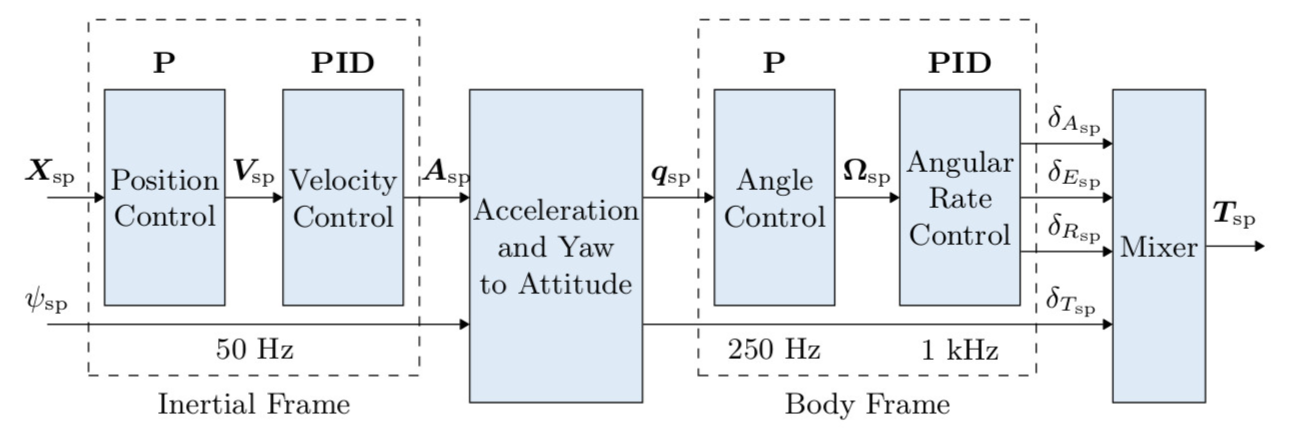
\includegraphics[scale=0.44]{obrazky/PX4CONTROLLER}
  \end{center}
  \caption[Řídící struktura systému PX4]{Řídící struktura systému PX4. \cite{PX4docs}}
  \label{fig:PX4controller}
\end{figure}

Zprávy typu \texttt{geometry\_msgs::msg::TwistStamped} jsou z nadřazeného uzlu publikovány do ROS 2 témy (\textit{topic}) \texttt{/mavros/setpoint\_velocity/cmd\_vel} s frekvencí 10 Hz.

\section{Mise pro sledování dynamického objektu}

Funkčnost simulace jsme také demonstrovali na složitější robotické misi jejímž cílem bylo sledování dynamického objektu. 

Pro tuto úlohu jsme využili data z měření radiace pomocí všesměrového radiačního detektoru, který byl umístěný na pozemním robotu. Robot pomocí částicového filtru (\textit{particle filter}) estimoval pozici radioaktivního zářiče a na základě této estimace se k zdroju radiace přibližoval. Celá mise byla prováděna v okolí Fakulty elektrotechniky a komunikačních technologií VUT v Brně.

Data z měření jsme měli k dispozici jako \texttt{rosbag} soubor\footnote{Rosbag soubor slouží na zálohu dat v podobě ROS 2 témat (\textit{topic})}, který obsahuje zprávy typu \texttt{geographic\_msgs::msg::GeoPoseStamped} a publiku je do ROS 2 tématu \texttt{/estimated\_source\_location}. Tyto zprávy obsahují globální souřadnice estimovaného zdroje radiace podle standardu WGS 84. Dron se v průběhu celé mise pohybuje v konstantní výšce, která de definovatelná uživatelem pomocí ROS 2 parametru.

Na obrázku \ref{fig:SIM3QGC} je zobrazený software QGroundControl s trajektorii mise pro sledování dynamického objektu. V levém horním rohu můžeme vidět, že dron je přepnutý do \textit{offboard} letového režimu. Jak je možné vidět na obrázku, simulovaná mise byla prováděna taky v okolí Fakulty elektrotechniky a komunikačních technologií VUT v Brně. Počáteční souřadnice mise byla 49.22812907° severní šířky, 16.57222321° východní délky, v nadmořské výšce 283 metrů.

\begin{figure}[!ht]
  \begin{center}
    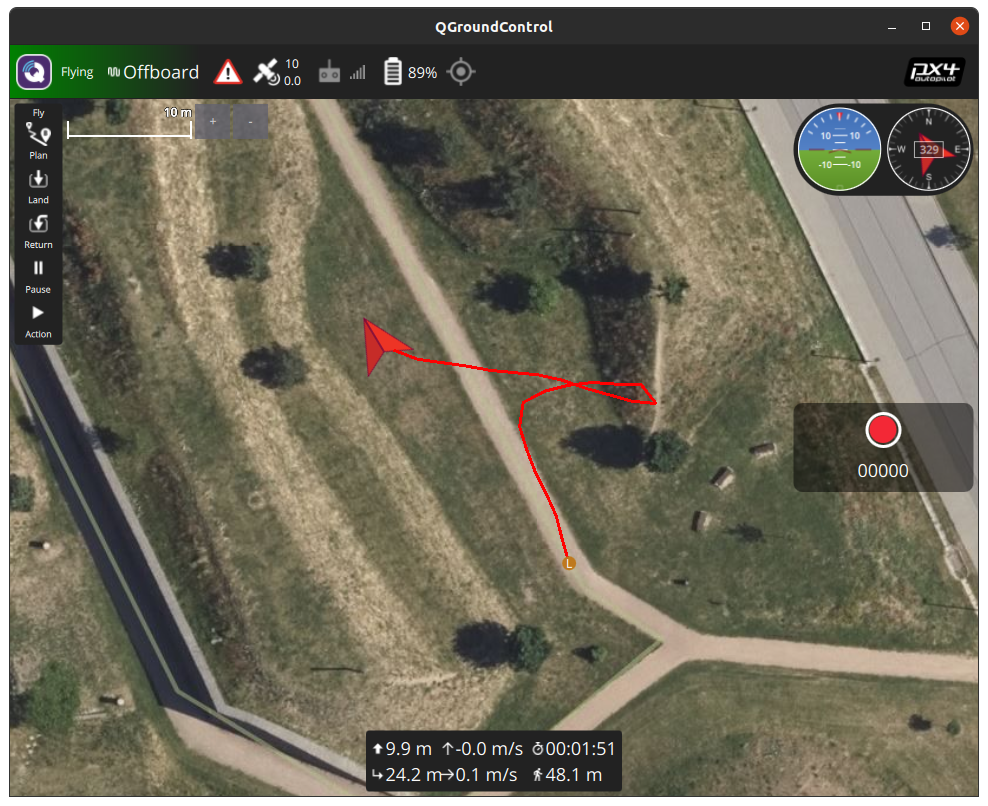
\includegraphics[scale=0.40]{obrazky/MISESL1}
  \end{center}
  \caption[Mise pro sledování dynamického objektu v software QGroundControl]{Mise pro sledování dynamického objektu v software QGroundControl.}
  \label{fig:SIM3QGC}
\end{figure}

Obrázek \ref{fig:SIM3GAZ} zobrazuje vzlet dronu v průběhu simulované mise pro sledování dynamického objektu v robotickém simulačním prostředí Gazebo 11.

\begin{figure}[!ht]
  \begin{center}
    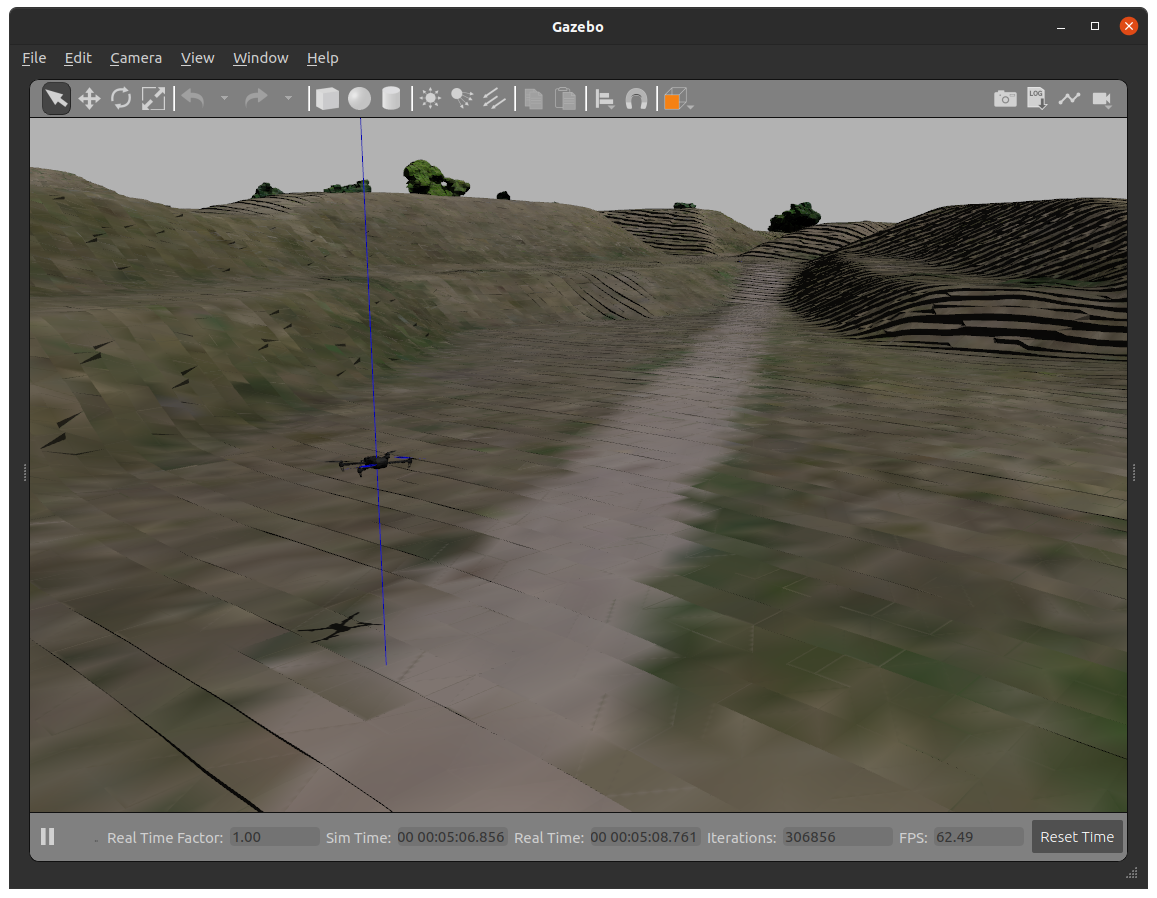
\includegraphics[scale=0.35]{obrazky/GAZSIMPLE.png}
  \end{center}
  \caption[Mise pro sledování dynamického objektu v simulačním software Gazebo 11]{Mise pro sledování dynamického objektu v simulačním software Gazebo 11.}
  \label{fig:SIM3GAZ}
\end{figure}


\section{Simulace misí s více drony}

Dalším z cílů práce bylo zobecnit navržené řešení tak, aby bylo možné simulovat mise s více bezpilotními letadly najednou. Z důvodu modularity systému ROS (ROS 2) nebyla tato úloha složitá. Pomocí \texttt{.launch} souboru jsme nadefinovali všechny ROS 2 uzly, které se mají spustit. Ke každému uzlu je nadefinovaný ROS 2 \texttt{namespace} tak, aby každý uzel pro řízení mise komunikoval se správným Mavros uzlem a tím taky se správným simulovaným dronem.

\subsection{Mise pro sledování dynamického objektu s více drony}

Obrázek \ref{fig:SIM3MULQG} 

DOKONCIT

\begin{figure}[!ht]
  \begin{center}
    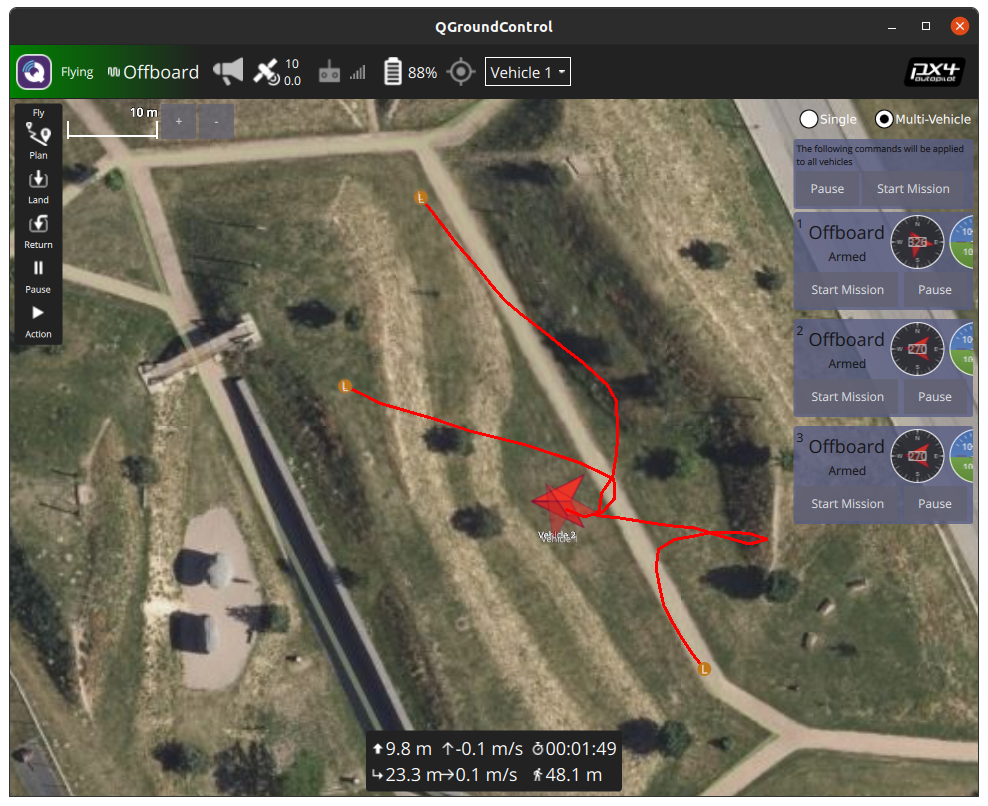
\includegraphics[scale=0.41]{obrazky/QGMULTIPLE.png}
  \end{center}
  \caption[Mise pro sledování dynamického objektu s více drony v software QGroundControl]{Mise pro sledování dynamického objektu s více drony v software QGroundControl.}
  \label{fig:SIM3MULQG}
\end{figure}

Obrázek \ref{fig:SIM3MULGAZ}

DOKONCIT

\begin{figure}[!ht]
  \begin{center}
    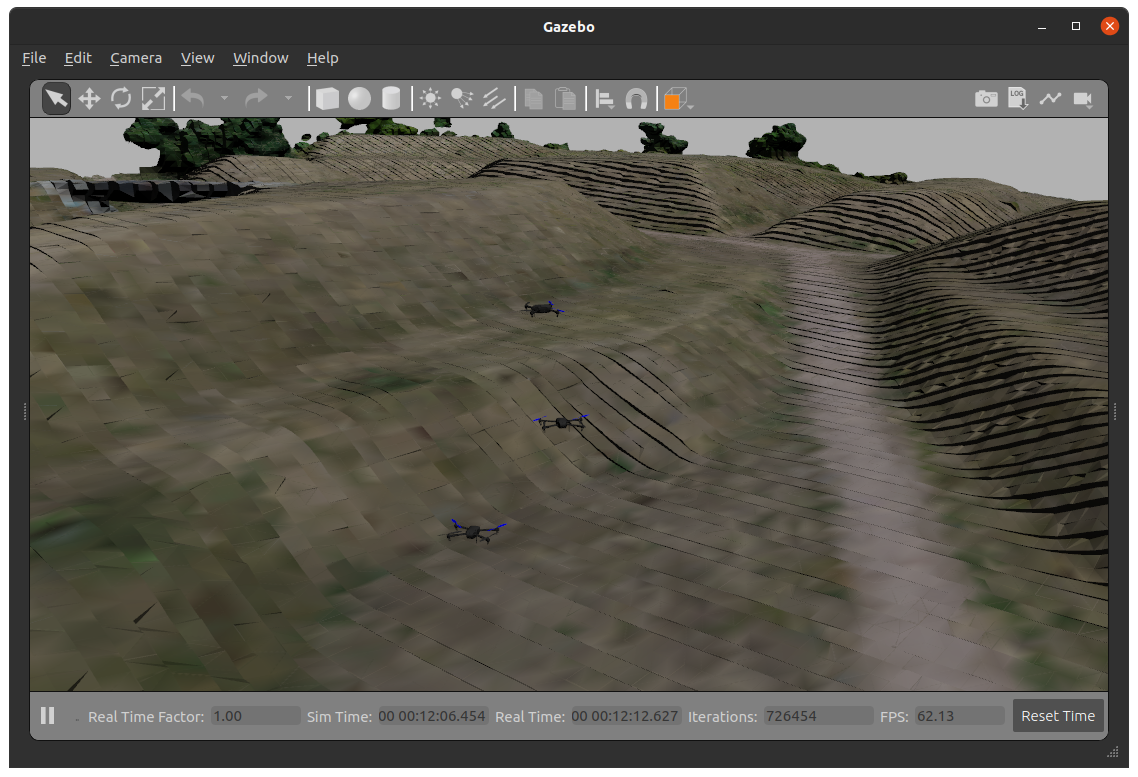
\includegraphics[scale=0.38]{obrazky/GAZMULTIPLE.png}
  \end{center}
  \caption[Mise pro sledování dynamického objektu s více drony v software Gazebo 11]{Mise pro sledování dynamického objektu s více drony v software Gazebo 11.}
  \label{fig:SIM3MULGAZ}
\end{figure}
